\documentclass[hyperref,UTF8]{article}
\usepackage{ctex}
\usepackage[margin=1in]{geometry}
\usepackage{booktabs}
\usepackage{bigstrut}
\usepackage{caption}
\usepackage{amsmath}
\usepackage{graphicx, subfig}
\usepackage{float}
\usepackage{color}
\usepackage{colortbl}
\usepackage{listings}
  \usepackage{textcomp} % 必须加上,否则报错
  \usepackage[framed,numbered,autolinebreaks,useliterate]{mcode}    % 添加matlab代码宏
  \usepackage{xcolor}
  \lstset{
  language=Matlab,  %代码语言使用的是matlab
  rulesepcolor=\color{red!20!green!20!blue!20},%代码块边框为淡青色
  keywordstyle=\color{blue!90}\bfseries, %代码关键字的颜色为蓝色,粗体
    numbers=left, % 显示行号
    numberstyle=\tiny,    % 行号字体
   commentstyle=\color[RGB]{0,130,0},    % 设置代码注释的颜色
  showstringspaces=false,%不显示代码字符串中间的空格标记
  stringstyle=\ttfamily, % 代码字符串的特殊格式
  breaklines=true, %对过长的代码自动换行
  extendedchars=false,  %解决代码跨页时,章节标题,页眉等汉字不显示的问题
  escapeinside=``,      % 代码中出现中文必须加上,否则报错
  texcl=true,}
  \lstset{breaklines}
\usepackage[framed,numbered,autolinebreaks,useliterate]{mcode}
\usepackage[colorlinks,linkcolor=black,
            anchorcolor=blue,
            citecolor=black]{hyperref}
\renewcommand\appendix{\setcounter{secnumdepth}{-2}}
\usepackage{multirow}
\usepackage{type1cm}
\usepackage{indentfirst}
\usepackage{setspace}
\usepackage{CJK}
\usepackage{ifthen}
\usepackage{titlesec}
\usepackage{titletoc}
\titleformat{\section}{\centering\heiti\zihao{4}}{\thesection}{0.3em}{}
\titleformat{\subsection}{\heiti\zihao{-4}}{\thesubsection}{0.3em}{}
\titleformat{\subsubsection}{\heiti\zihao{-4}}{\thesubsubsection}{0.3em}{}
\newcommand{\CJKfontsize}[4]{%
\fontsize{#1}{#2 plus#3 minus #4}\selectfont}
\geometry{a4paper,left=2cm,right=2cm,top=1cm,bottom=1cm}
\zihao{-4}
\geometry{a4paper,left=3.18cm,right=3.18cm,top=2.54cm,bottom=2.54cm}
\begin{document}
%\thispagestyle{empty}
%\tableofcontents
%\thispagestyle{empty}
%\newpage\setcounter{page}{1}

\newpage\setcounter{page}{1}
\setlength{\baselineskip}{14pt}\zihao{-4}\songti{

\section{问题重述}
\subsection{问题背景}
随着现代机械加工工业的发展,无论是在大中型制造企业还是传统加工企业,对玻璃、金属、木板、塑料、面料等原材料的切割加工问题涉及到工艺、家具、电子、装饰等众多领域。为了减少生产成本,增加企业利润,就需要通过更合理的切割方式来提高原料的利用率,尽可能的减少下料。如若仅凭借个人经验排料则会导致原材料利用率低、工作效率低下、成本增加。因此我们需要通过已知的板材数据和企业生产计划来制定合理高效的下料切割计划、进行板材定额及生产成本计算,为材料库准备材料提供计划,为企业经管部门提供决策依据和材料采购预算。
\subsection{需要解决的问题}
徐州一家具厂新进了一批木板原材料,已知板材原料S1及各待加工产品的信息,忽略木板厚度和切割缝宽,编制出与生产任务和利润相匹配的板材切割列表。
\begin{enumerate}
\item 在一块S1上只切割P1,求木板利用率最大时切割的P1数量及该最大利用率值。
\item 在一块S1上同时切割P1、P3,求木板利用率按从高到低顺序排名前三的切割方案及利用率值。
\item 在完成给定的P1、P3生产任务的基础上,求出木板总利用率最高时的切割方案及利用率值。
\item 在完成给定的P1、P2、P3、P4生产任务的基础上,求出木板总利用率最高时的切割方案及最大总利用率值。
\item 在100张S1上切割P1、P2、P3、P4,求所获利润最大时的切割方案及总利用率值。
\end{enumerate}

\section{模型假设}
\begin{enumerate}
\item 假设切割过程无木板损耗;
\item 假设不考虑切割工具的厚度;
\item 假设切割工具可旋转;
\item 假设题目所给的数据真实可靠;
\end{enumerate}

\section{符号说明}
\begin{table}[htbp]
\centering
\caption{本文中所涉及的符号及说明}\label{abs}
\begin{tabular}{|c|c|}
\hline
符号&意义\\
\hline
$L$ & 木板原材料S1的长度 \\
$W$ & 木板原材料S1的宽度 \\
$l_i$ & 小矩形产品$P_i$的长度 \\
 $w_i$& 小矩形产品$P_i$的宽度 \\
$E$ & 木板利用率 \\
$x_i$ & 产品$P_i$在S1排样时左下角点的横坐标 \\
$y_i$ & 产品$P_i$在S1排样时左下角点的纵坐标 \\
$n_{P1}$ & P1的生产任务数量 \\
 $n_{P2}$& P2的生产任务数量 \\
$n_{P3}$ & P3的生产任务数量 \\
$n_{P4}$ & P4的生产任务数量 \\
$A_{P1}$ & P1的面积 \\
$A_{P2}$ & P2的面积 \\
 $A_{P3}$& P3的面积 \\
 $A_{P4}$& P4的面积 \\
$N$ & 需要木板S1的块数 \\
 $ k_i$& 按第i种方案切割的木板块数 \\
$M$& 总利润 \\\hline
\end{tabular}%
\end{table}

\section{问题分析与求解}


\subsection{问题一、二的分析与求解}
\subsubsection{问题分析}
设矩形木板S1长度为$L$,宽度为$W$,根据题目所给条件已知$L=3000mm$,$W=1500mm$。以S1为原材料,问题一在一块矩形木板S1上切割面积更小的矩形产品 P1 ,问题二在一块矩形木板S1上切割面积更小的矩形产品 P1,P3 。设该矩形产品的长度为$l_i$,宽度为$w_i$,切割n个小矩形产品,则木板利用率为
\begin{equation}\label{liyongligongshi}
  E=\frac{\sum_{i=1}^{n}{l_iw_i}}{LW}
\end{equation}
由于两问均是在大矩形木板上切割小矩形产品,假设忽略切割木材过程中的损耗,因此都可以看作二维矩形排样问题。两问区别仅在于问题一的矩形件集合全为P1,而问题二的矩形件集合为P1和P3排列。\par 因此,我们建立同一个模型来解决问题一和问题二。\par
题目要求木板利用率最大,因此我们以木板利用率为最优指标函数,建立一个动态规划模型。基于剩余矩形匹配法,建立二维动态坐标 ,代表第i个矩形放入S1的位置,加以约束条件,进行决策,并以模拟退火算法改进了剩余矩形法,计算得到最大木板利用率时的板材切割方案,达到全局最优。其过程见图\ref{paiyang}。
\begin{figure}[htbp]
  \centering
  \includegraphics[width=0.8\textwidth]{picture/liucheng}
  \caption{矩形排样决策过程图}\label{paiyang}
\end{figure}
\subsubsection{问题一、二的模型建立与求解}
动态规划是解决多阶段决策过程最优化的一种数学方法。将产品$P_i$不断往木板S1上排样的过程即可看作一个多阶段决策过程,在每个阶段开始时,产品$P_i$根据剩余矩形状态进行决策,选择在哪个矩形下料,决策完成后进入下一阶段。\\
\ \\
\textbf{剩余矩形法}\par
设原料的左下角和右上角的坐标分别为$(x_0,y_0),(x_1,y_1)$,所有下一个下料点都是以剩余矩形的左下角开始。设下料零件$P_i$ 的长宽尺寸分别为$l_0,w_0$,则下料后的两个剩余矩形为$[ (x_0,y_0+w_0),(x_1,y_1)]$、$[(x_0+l_0,y_0),(x_1,y_1)]$,选择一个矩形后,继续下料。如图\ref{shengyujuxing}
所示\cite{1}。
\begin{figure}[htbp]
  \centering
  \includegraphics[width=.8\textwidth]{picture/PIC}
  \caption{剩余矩形匹配法图示}\label{shengyujuxing}
\end{figure}\\
\ \\
\textbf{基于剩余矩形法的动态规划模型}\par
本模型所涉及的动态规划概念如下:
\subparagraph{阶段}
将问题的过程恰当地分为若干个相互联系的阶段。在第n次切割完后,产生n+1个矩形。记在n+1个矩形中选择一个,并将$P_{i+1}$放入选中矩形排样为一个阶段。
\subparagraph{状态}
表示每个阶段开始时所处的客观条件,描述各个状态的变量称为状态变量。每个产品排样后,产品的空间坐标即为状态。\par
对于一种矩形产品在木板原材料上的排列有两种方式:一是产品的长与原材料的长平行,产品宽与原材料的宽平行;二是产品的长与原材料的宽平行,产品宽与原材料的长平行。参见图\ref{py-long}及图\ref{py-long2}。\par
\begin{figure}[htbp]
  \centering
  \includegraphics[width=.7\textwidth]{picture/PPT1}
  \caption{长平行长排列的坐标图}\label{py-long}
\end{figure}
\begin{figure}[htbp]
  \centering
  \includegraphics[width=.7\textwidth]{picture/PPT2}
  \caption{长平行宽排列的坐标图}\label{py-long2}
\end{figure}
\subparagraph{决策}当处于阶段的某个状态时,从该状态做出某个选择可以演变到下一状态,这种选择称为决策。该决策需满足以下条件:
\begin{enumerate}
  \item 根据产生的矩形数据,判断图形关系,将待排样产品长度与n+1个矩形长宽相比,选出比值最大的方案进行排样。
  \item 排列时任意两个矩形之间不能有重叠;
  \item 矩形产品不能排列到板材原材料之外;
\end{enumerate}
即用公式表述如式(\ref{PRO1_1})及式(\ref{PRO1_2})。\\
方式一排列:
\begin{equation}\label{PRO1_1}
\begin{split}
&s.t.\quad  \left\{\begin{array}{c}
\sum_{i=1}^n l_iw_i\leq LW\quad\\
0\leq x_i\leq L\quad \\
0\leq y_i\leq W\quad \\
0\leq x_i+l_i\leq L\quad \\
0\leq y_i+w_i\leq W\quad \\
\end{array}\right.
\end{split}
\end{equation}
方式二排列:
\begin{equation}\label{PRO1_2}
\begin{split}
&s.t.\quad  \left\{\begin{array}{c}
\sum_{i=1}^n l_iw_i\leq LW\quad\\
0\leq x_i\leq L\quad \\
0\leq y_i\leq W\quad \\
0\leq x_i+w_i\leq L\quad \\
0\leq y_i+l_i\leq W\quad \\
\end{array}\right.
\end{split}
\end{equation}
\subparagraph{最优指标函数}
动态规划中衡量决策结果的指标称为指标函数。在此模型中求木板利用率最大,因此我们以木板利用率式(\ref{liyongligongshi})为最优指标函数。
\subparagraph{策略}
按某一顺序排列的决策称为一个策略,能达到最优效果的策略称为最优策略。\\
\ \\
\textbf{模拟退火算法}\par
根据以上函数及其约束条件,我们采取模拟退火算法对其进行求解。模拟退火算法是一种在全局寻求最优解的策略\cite{2},将式(\ref{liyongligongshi})作为目标函数,则目标函数值越大,木板利用率越高。模拟退火算法的算法框图如图\ref{kuangtu1}
所示。
\begin{figure}[htbp]
  \centering
  \includegraphics[width=.6\textwidth]{picture/liuchengway2}
  \caption{模拟退火剩余矩形算法流程图}\label{kuangtu1}
\end{figure}\par
降温方式对模拟退火算法优化结果有很大影响。如果温度下降过快,可能会丢失极值点;反之,则大大降低算法的收敛速度。本文定义的降温公式为
\begin{equation}\label{tuihuowendu}
T(K)=\frac{T_0}{k^m},k=1,2,\cdots
\end{equation}
其中  $T_0>0$为初始温度,$T(k)$为当第k次迭代的温度,m为大于等于1的常数。当满足条件:温度达到终止温度时,算法终止。\par
\subsubsection{问题一、二的结果}
经过运算后得到问题一的答案见表\ref{tab:P11},切割方案见图\ref{probelem1}
;问题二的答案见表\ref{tab:addlabela}
,切割方案见图\ref{probelem11}
至图\ref{probelem13}
。
\begin{table}[htbp]
  \centering
  \caption{\textbf{问题一的结果}}
    \begin{tabular}{|c|c|}
    \hline
    P1的数量 & 木板利用率 \\\hline
    59个 & 98.298\% \\\hline
    \end{tabular}%
  \label{tab:P11}%
\end{table}%
\begin{figure}[htbp]
  \centering
  \includegraphics[width=\textwidth]{picture/problem1}
  \caption{问题一的切割方案图示}\label{probelem1}
\end{figure}

\begin{table}[htbp]
  \centering
  \caption{\textbf{问题二的结果}}
    \begin{tabular}{|c|c|c|c|}
    \hline
    方案编号& P1的数量 & P3的数量 & 木板利用率\\
    \hline
    1 & 44 & 12 & 98.100\% \\
    \hline
    2 & 45 & 11 & 97.700\% \\
    \hline
    3 & 35 & 19 & 97.568\% \\
    \hline
    \end{tabular}%
  \label{tab:addlabela}%
\end{table}%
\begin{figure}[htbp]
  \centering
  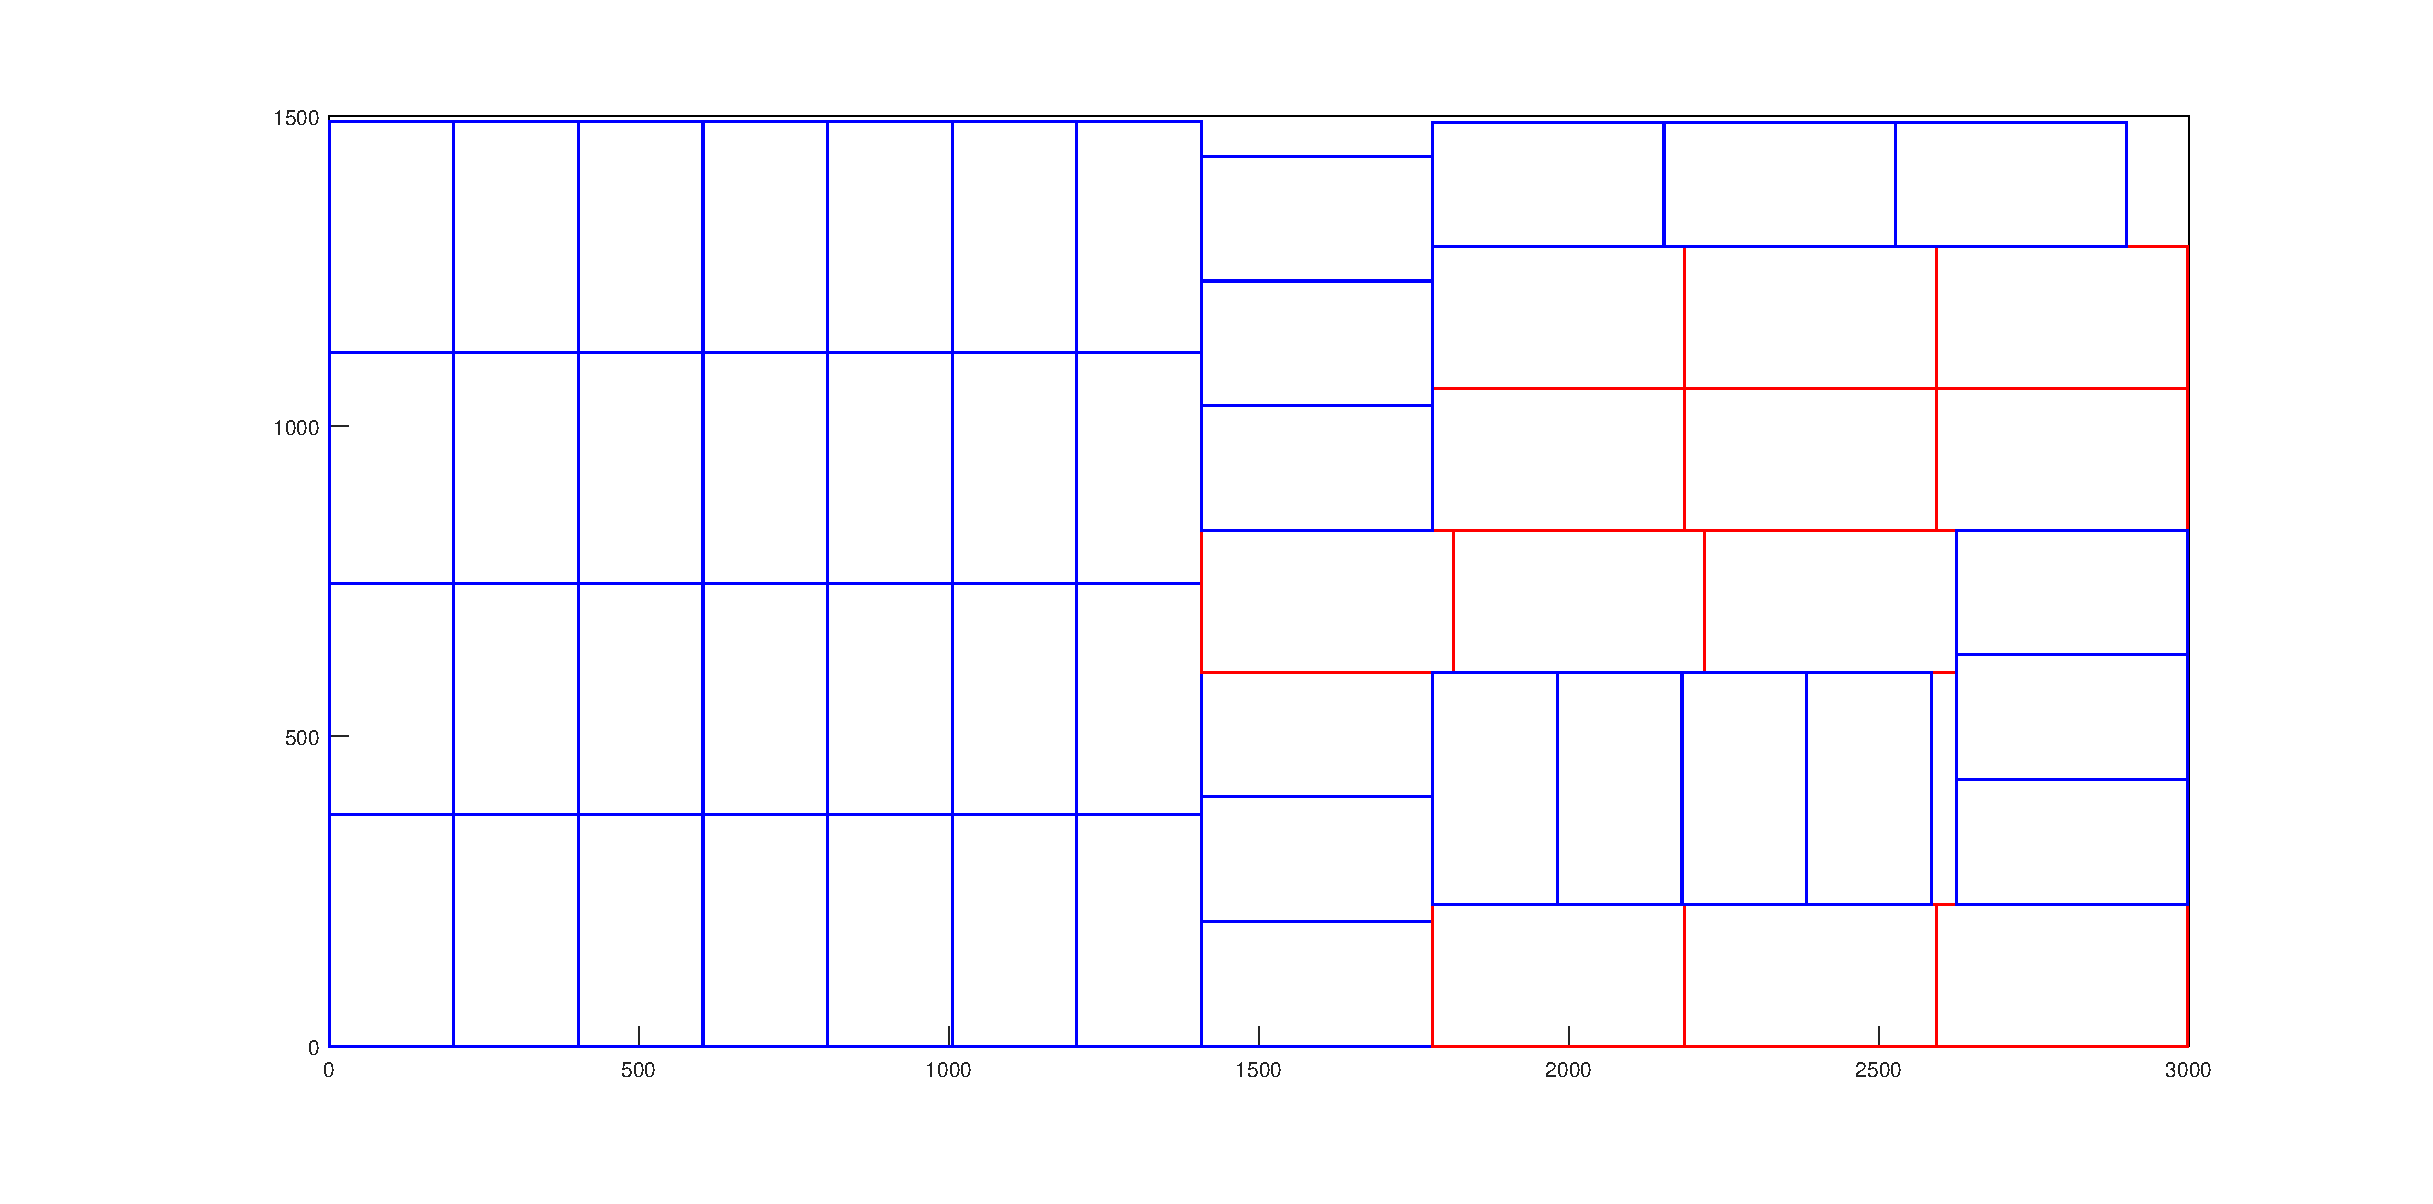
\includegraphics[width=\textwidth]{picture/P_2_44_12}
  \caption{问题二方案一的切割图示}\label{probelem11}
\end{figure}
\begin{figure}[htbp]
  \centering
  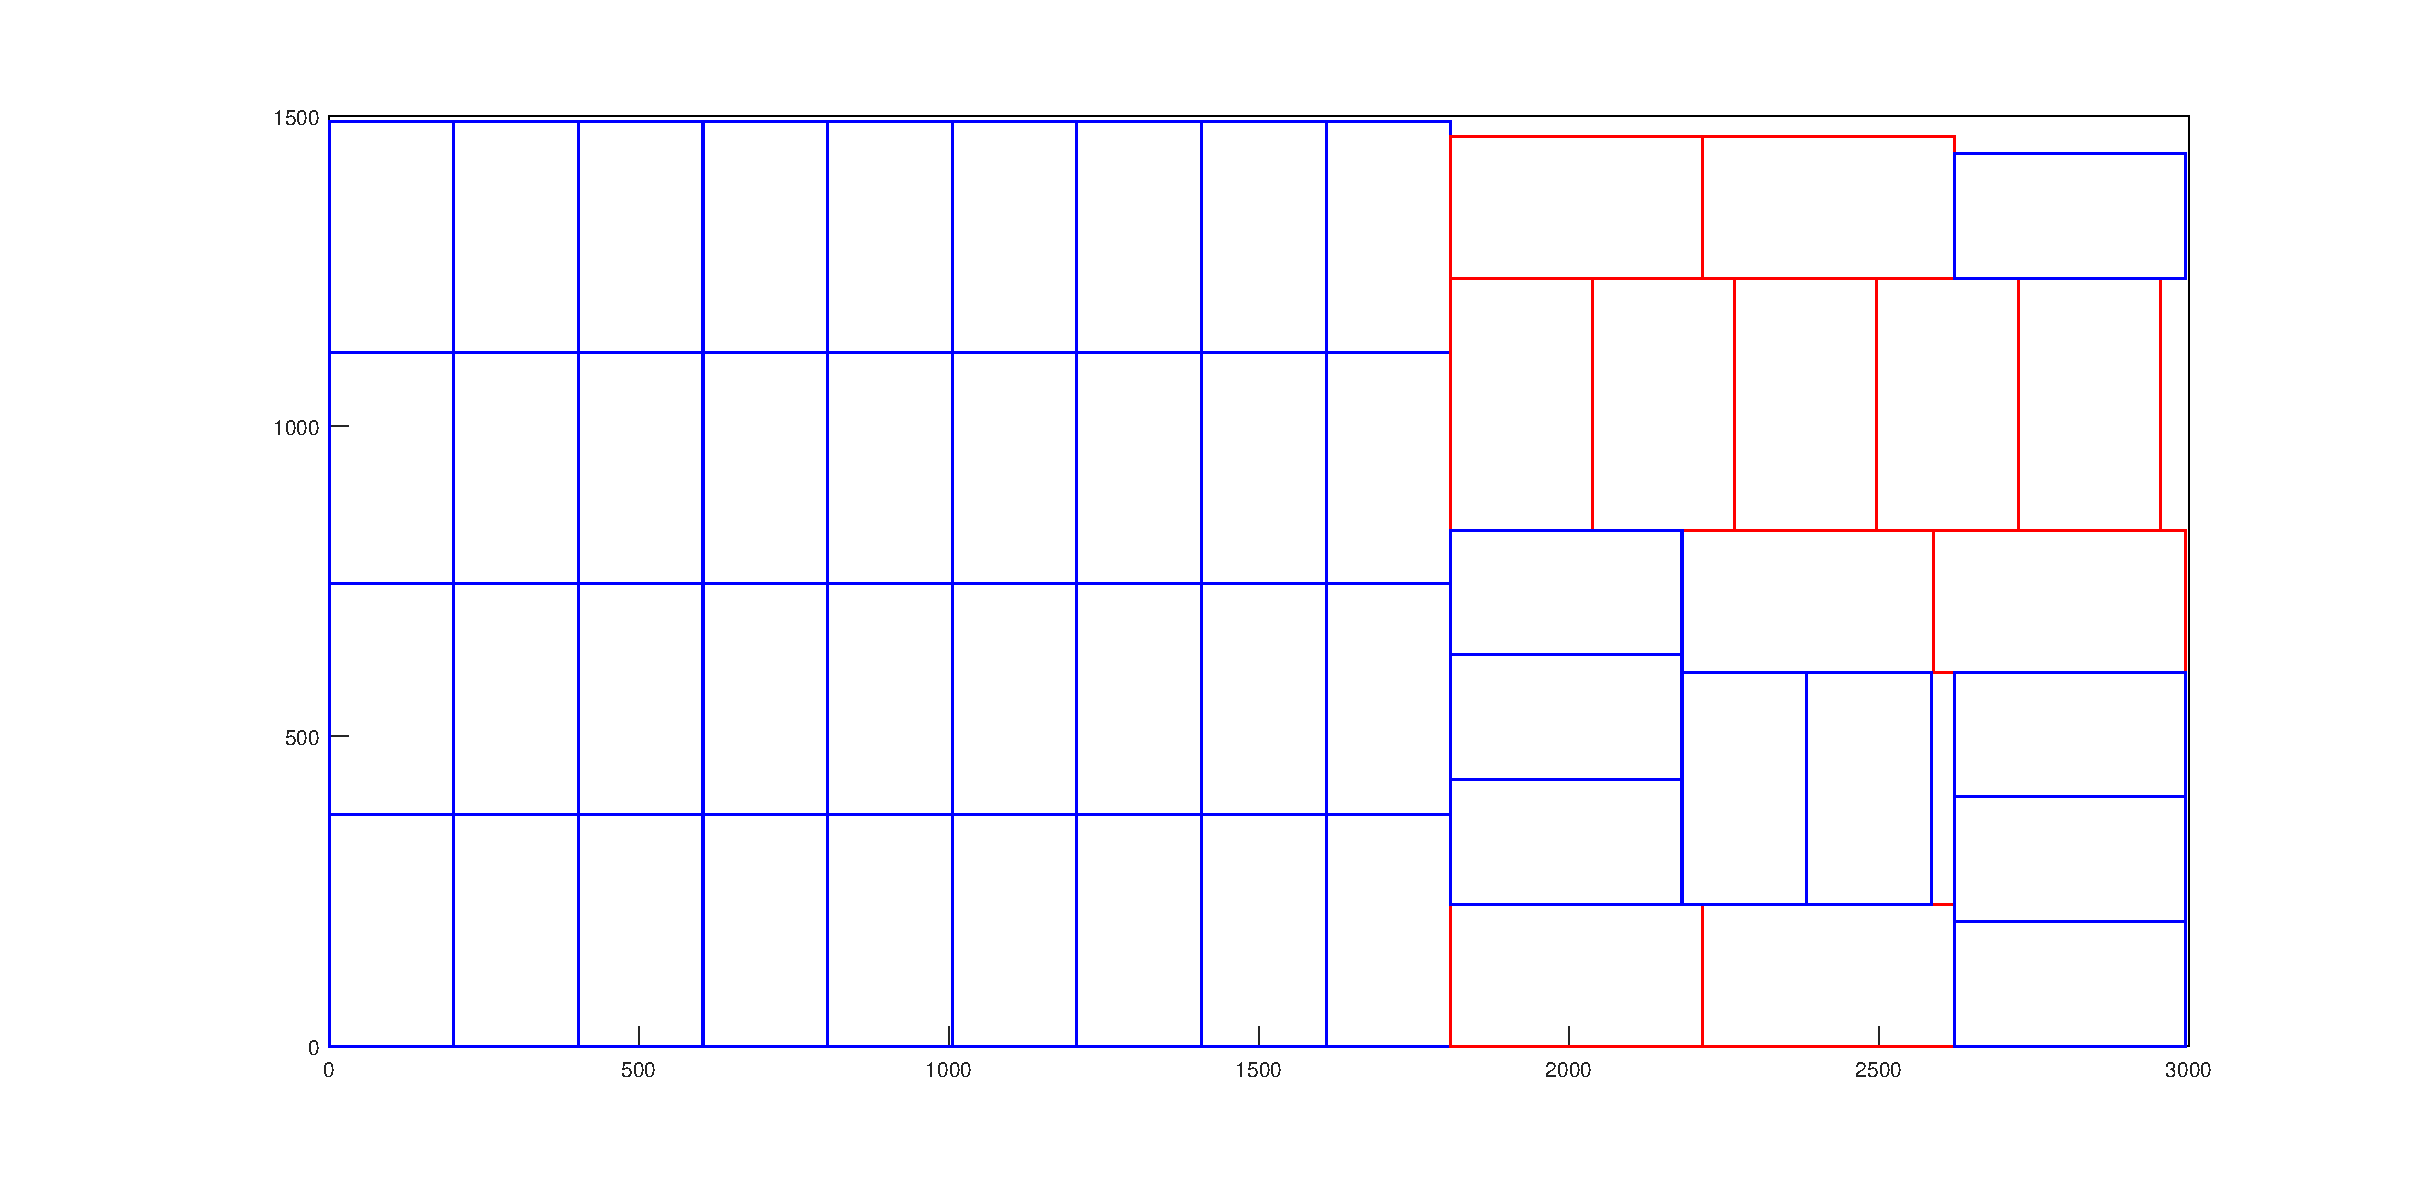
\includegraphics[width=\textwidth]{picture/P_2_45_11}
  \caption{问题二方案二的切割图示}\label{probelem12}
\end{figure}
\begin{figure}[htbp]
  \centering
  \includegraphics[width=\textwidth]{picture/P_2_35_19}
  \caption{问题二方案三的切割图示}\label{probelem13}
\end{figure}
\subsection{问题三、四的分析与求解}
\subsubsection{问题分析}
根据问题二的运算结果,我们得到了在一块木板原材料排列P1、P3产品使得木板利用率尽可能大的7种方案,按木板利用率从高到低排序见表\ref{tab:gaoliyonglv}。\par
\begin{table}[htbp]
  \centering
  \caption{在一块S1切割P1、P3的高利用率方案}
    \begin{tabular}{|c|c|c|c|}
    \hline
    方案编号 &P1的数量&P3的数量&木板利用率\\\hline
    1 & 59 & 0 & 98.298\% \\\hline
    2 & 44 & 12 & 98.100\% \\\hline
    3 & 45 & 11 & 97.700\% \\\hline
    4 & 35 & 19 & 97.568\% \\\hline
    5 & 0 & 47 & 97.106\% \\\hline
    6 & 16 & 34 & 96.904\% \\\hline
    7 & 32 & 21 & 96.702\% \\\hline
    \end{tabular}%
  \label{tab:gaoliyonglv}%
\end{table}%
而问题三和问题四将我们能用的木板数量从一块扩展到多块,问题三在达到P1、P3的生产任务数量:$n_{P1}=774\mbox{,}n_{P3}=1623$的条件下,使所有木板总利用率最高;问题四为在达到P1、P2、P3、P4的生产数量:$n_{P1}=774\mbox{,} n_{P2}=5153\mbox{,}n_{P3}=1623\mbox{,}n_{P4}=1614$ 的条件下,使所有木板总利用率最高。因此,我们建立同一个模型来解决问题三和问题四,参照问题二,我们同样能计算出在一块木板上切割P1、P2、P3、P4产品使得该木板利用率较高的25种方案,按照利用率值由高到低排序见表\ref{tab:haoliyong}。\par
\begin{table}[htbp]
  \centering
  \caption{一块S1上切割P1、P2、P3、P4的高利用率方案}
    \begin{tabular}{|c|c|c|c|c|c|}
    \hline
    序号 & P1 & P2 & P3 & P4 & 利用率 \\
    \hline
    1 & 3 & 5 & 27 & 15 & 99.054\% \\
    \hline
    2 & 0 & 2 & 45 & 0 & 98.952\% \\
    \hline
    3 & 0 & 0 & 41 & 9 & 98.705\% \\
    \hline
    4 & 40 & 5 & 6 & 3 & 98.650\% \\
    \hline
    5 & 1 & 6 & 36 & 3 & 98.645\% \\
    \hline
    6 & 24 & 4 & 0 & 30 & 98.592\% \\
    \hline
    7 & 12 & 9 & 25 & 0 & 98.548\% \\
    \hline
    8 & 59 & 0 & 0 & 0 & 98.298\% \\
    \hline
    9 & 0 & 8 & 36 & 0 & 98.293\% \\
    \hline
    10 & 0 & 0 & 43 & 6 & 98.172\% \\
    \hline
    11 & 36 & 6 & 6 & 5 & 98.085\% \\
    \hline
    12 & 0 & 10 & 33 & 0 & 98.073\% \\
    \hline
    13 & 45 & 7 & 1 & 0 & 97.963\% \\
    \hline
    14 & 48 & 6 & 0 & 0 & 97.906\% \\
    \hline
    15 & 10 & 10 & 0 & 33 & 97.868\% \\
    \hline
    16 & 0 & 14 & 12 & 20 & 97.742\% \\
    \hline
    17 & 33 & 11 & 1 & 5 & 97.702\% \\
    \hline
    18 & 0 & 4 & 12 & 39 & 97.395\% \\
    \hline
    19 & 0 & 18 & 0 & 28 & 97.346\% \\
    \hline
    20 & 16 & 6 & 24 & 2 & 97.288\% \\
    \hline
    21 & 9 & 19 & 4 & 11 & 97.159\% \\
    \hline
    22 & 0 & 0 & 47 & 0 & 97.106\% \\
    \hline
    23 & 0 & 8 & 0 & 47 & 96.999\% \\
    \hline
    24 & 0 & 24 & 6 & 8 & 96.577\% \\
    \hline
    25 & 20 & 21 & 0 & 0 & 96.095\% \\
    \hline
    \end{tabular}%
  \label{tab:haoliyong}%
\end{table}%
设产品P1的面积为$A_{P1}$,产品P2的面积为 $A_{P2}$,产品P3的面积为 $A_{P3}$,产品P4的面积为$A_{P4}$ ,木板原材料S1的面积为$A_{S1}$,需要的木板原材料数为$N$。 、 $A_{P1}\mbox{、}A_{P2}\mbox{、}A_{P3}\mbox{、}A_{P4}\mbox{、}A_{S1}$都为定值。\par
对于问题三:
$$\mbox{木板总利用率}=\frac{\mbox{所有产品的总面积}}{\mbox{所有木板的总面积}}=\frac{774\times A_{P1}+1623\times A_{P3}}{N\times A_{S1}}$$\par
对于问题四:
$$\mbox{木板总利用率}=\frac{\mbox{所有产品的总面积}}{\mbox{所有木板的总面积}}=\frac{774\times A_{P1}+2153\times A_{P2}+1623\times A_{P3}+1614\times A_{P4}}{N\times A_{S1}}$$\par
由于所有产品的总面积为一固定值,要得到最大的木板总利用率就要得到最小的所有木板总面积,即要求得使用木板的最小数量$N$。因此我们对单块木板利用率排名较高的几种方案进行组合,利用整数线性规划求得完成生产任务的条件下多块木板总利用率最高的组合方案。
\subsubsection{模型的建立与求解}
\paragraph{问题三的模型建立与求解}
设决策变量$k_i$为按第i种方案切割的木板块数($i=1,2,\cdots ,7$),则目标函数为使用木板原材料的最小值,由表\ref{tab:gaoliyonglv}可得:
\begin{equation}\label{zuixiaozhi1}
  \begin{split}
&\min \,\, N=\sum_{i=1}^7 k_i\\
&s.t.\quad  \left\{\begin{array}{c}
59k_1+44k_2+45k_3+35k_4+16k_6+32k_7\geq774\quad \\
12k_2+11k_3+19k_4+47k_5+34k_6+21k_7\geq1623\quad \\
k_i\geq0\mbox{且为整数}\quad \\
\end{array}\right.
\end{split}
\end{equation}
用Matlab对该整数线性规划问题求解,得到最优解为:$k_1=5,k_2=11,k_5=32$,其余为0,最小使用木板数N为48。于是问题三的结果见表\ref{tab:quastion3},以蓝色矩形代表P1,红色矩形代表P3,得到P1、P3在S1上的排样图见图\ref{qiegex1}
至图\ref{qiegex3}。
\begin{table}[htbp]
  \centering
  \caption{\textbf{问题三的结果}}
    \begin{tabular}{|c|c|c|c|c|}
    \hline
    木板S1 & P1& P3 & 木板 & \multicolumn{1}{c|}{\multirow{2}[0]{*}{备注}} \\
    的数量&   的数量&    的数量&     利用率      &\\\hline
    5 & 59 & 0 & 98.298\% & 每块木板切割方案相同 \\\hline
    11 & 44 & 12 & 98.100\% & 每块木板切割方案相同 \\\hline
    32 & 0 & 47 & 97.106\% & 每块木板切割方案相同 \\\hline
    合计数量: 48 & 774 & 1623 & 木板总利用率:96.725\% & 木板总利用率=$\frac{\mbox{所有产品的总面积}}{\mbox{所有木板的总面积}}$ \\\hline
    \end{tabular}%
  \label{tab:quastion3}%
\end{table}%
\begin{figure}[htbp]
  \centering
  \includegraphics[width=\textwidth]{picture/problem1}
  \caption{问题三$k_1$切割方案图示 }\label{qiegex1}
\end{figure}
\begin{figure}[htbp]
  \centering
  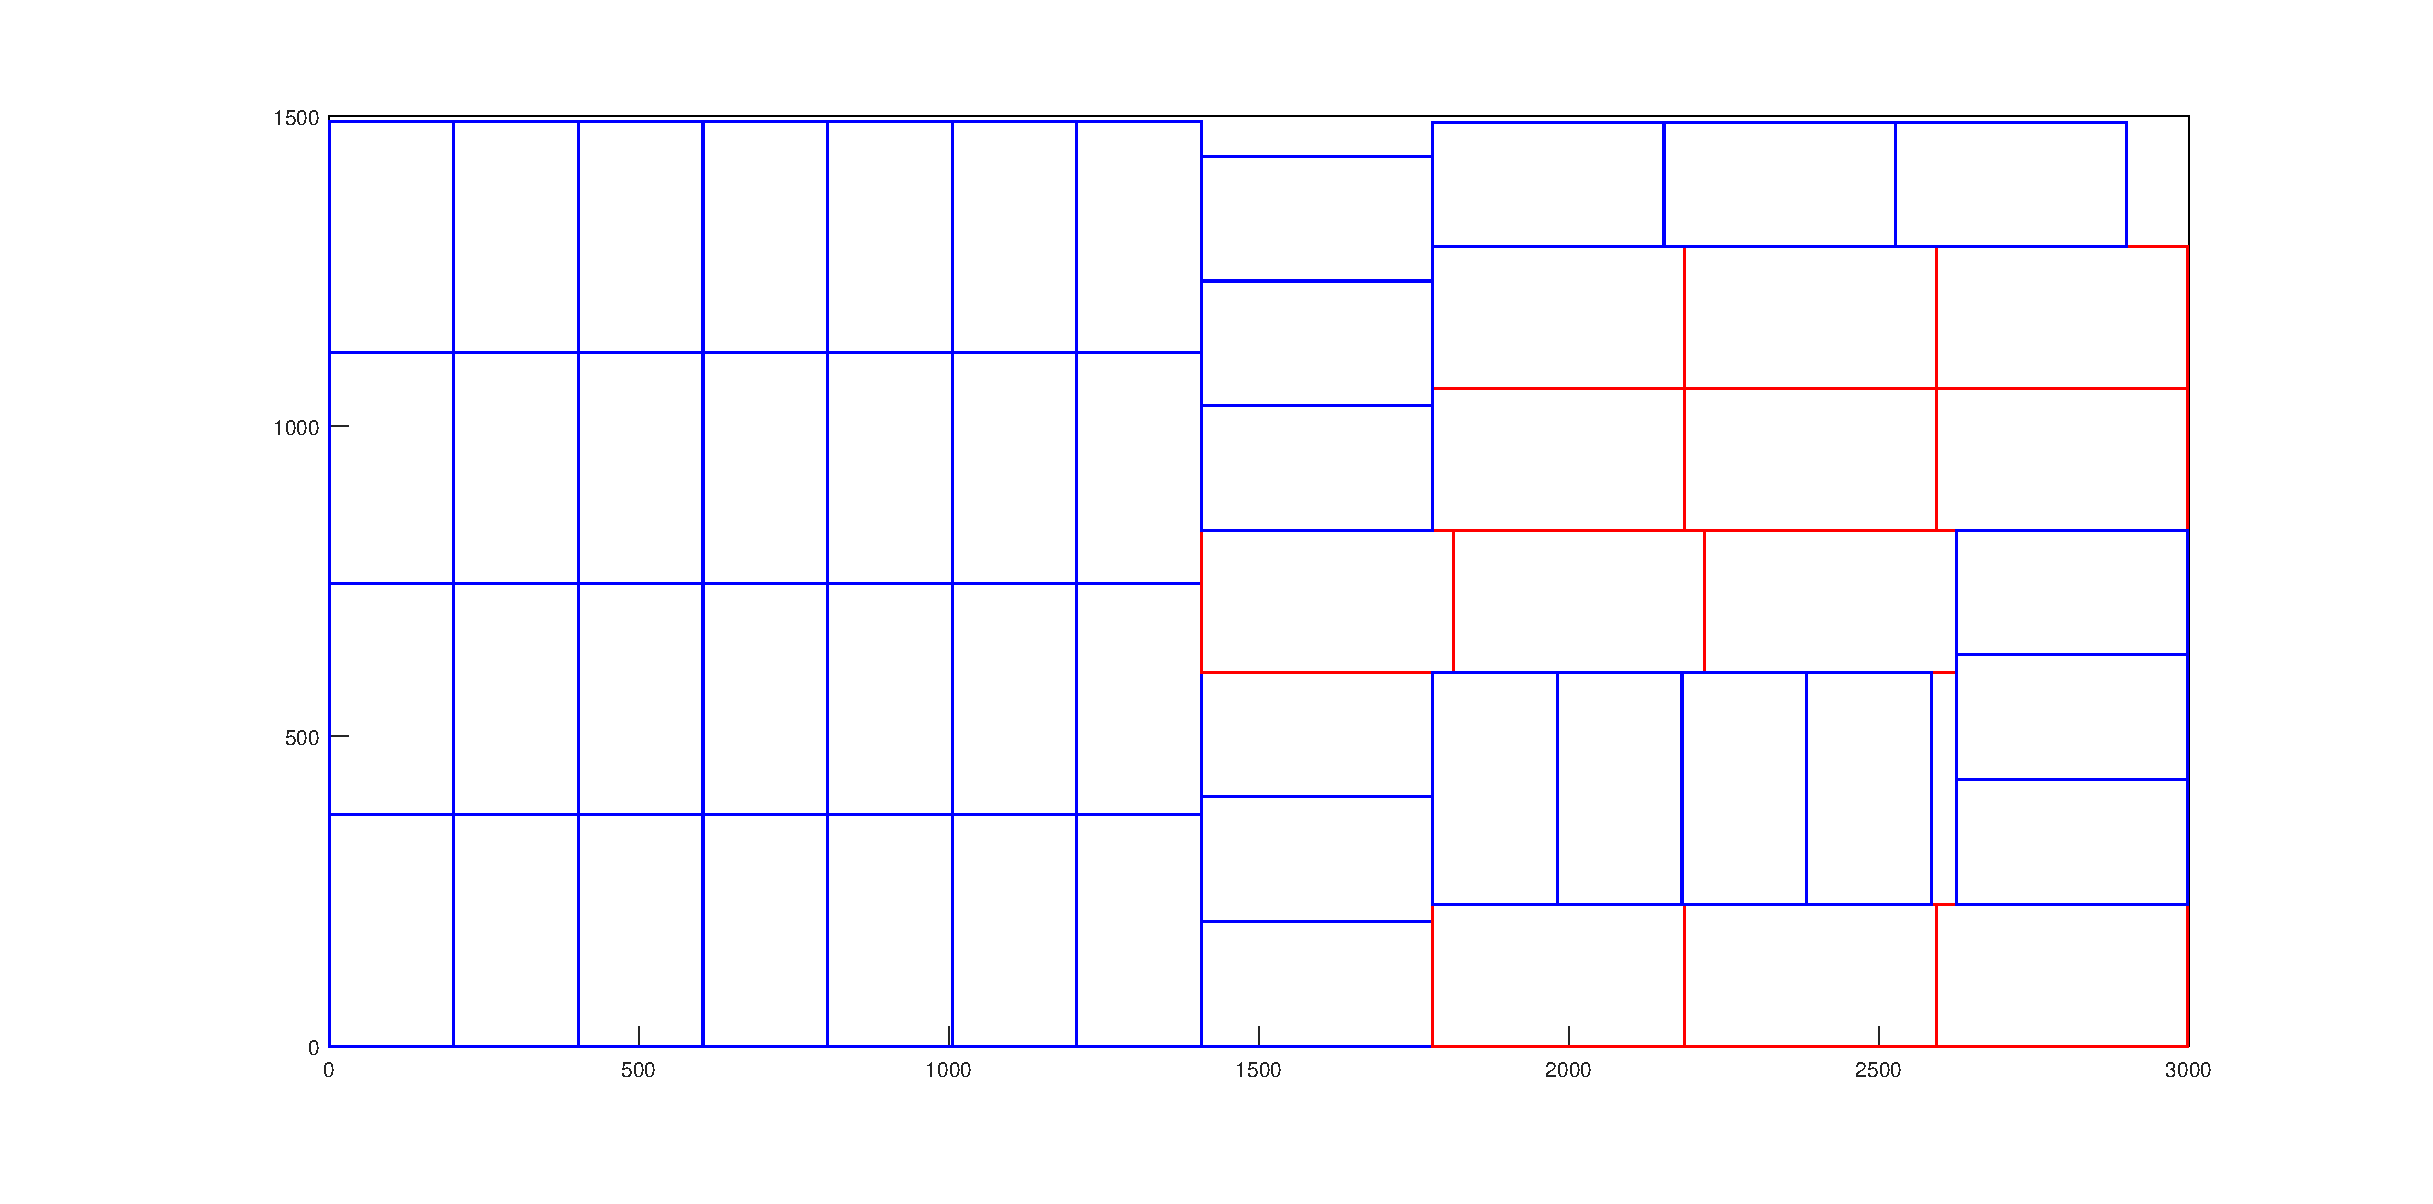
\includegraphics[width=\textwidth]{picture/P_2_44_12}
  \caption{问题三$k_2$切割方案图示 }\label{qiegex2}
\end{figure}
\begin{figure}[htbp]
  \centering
  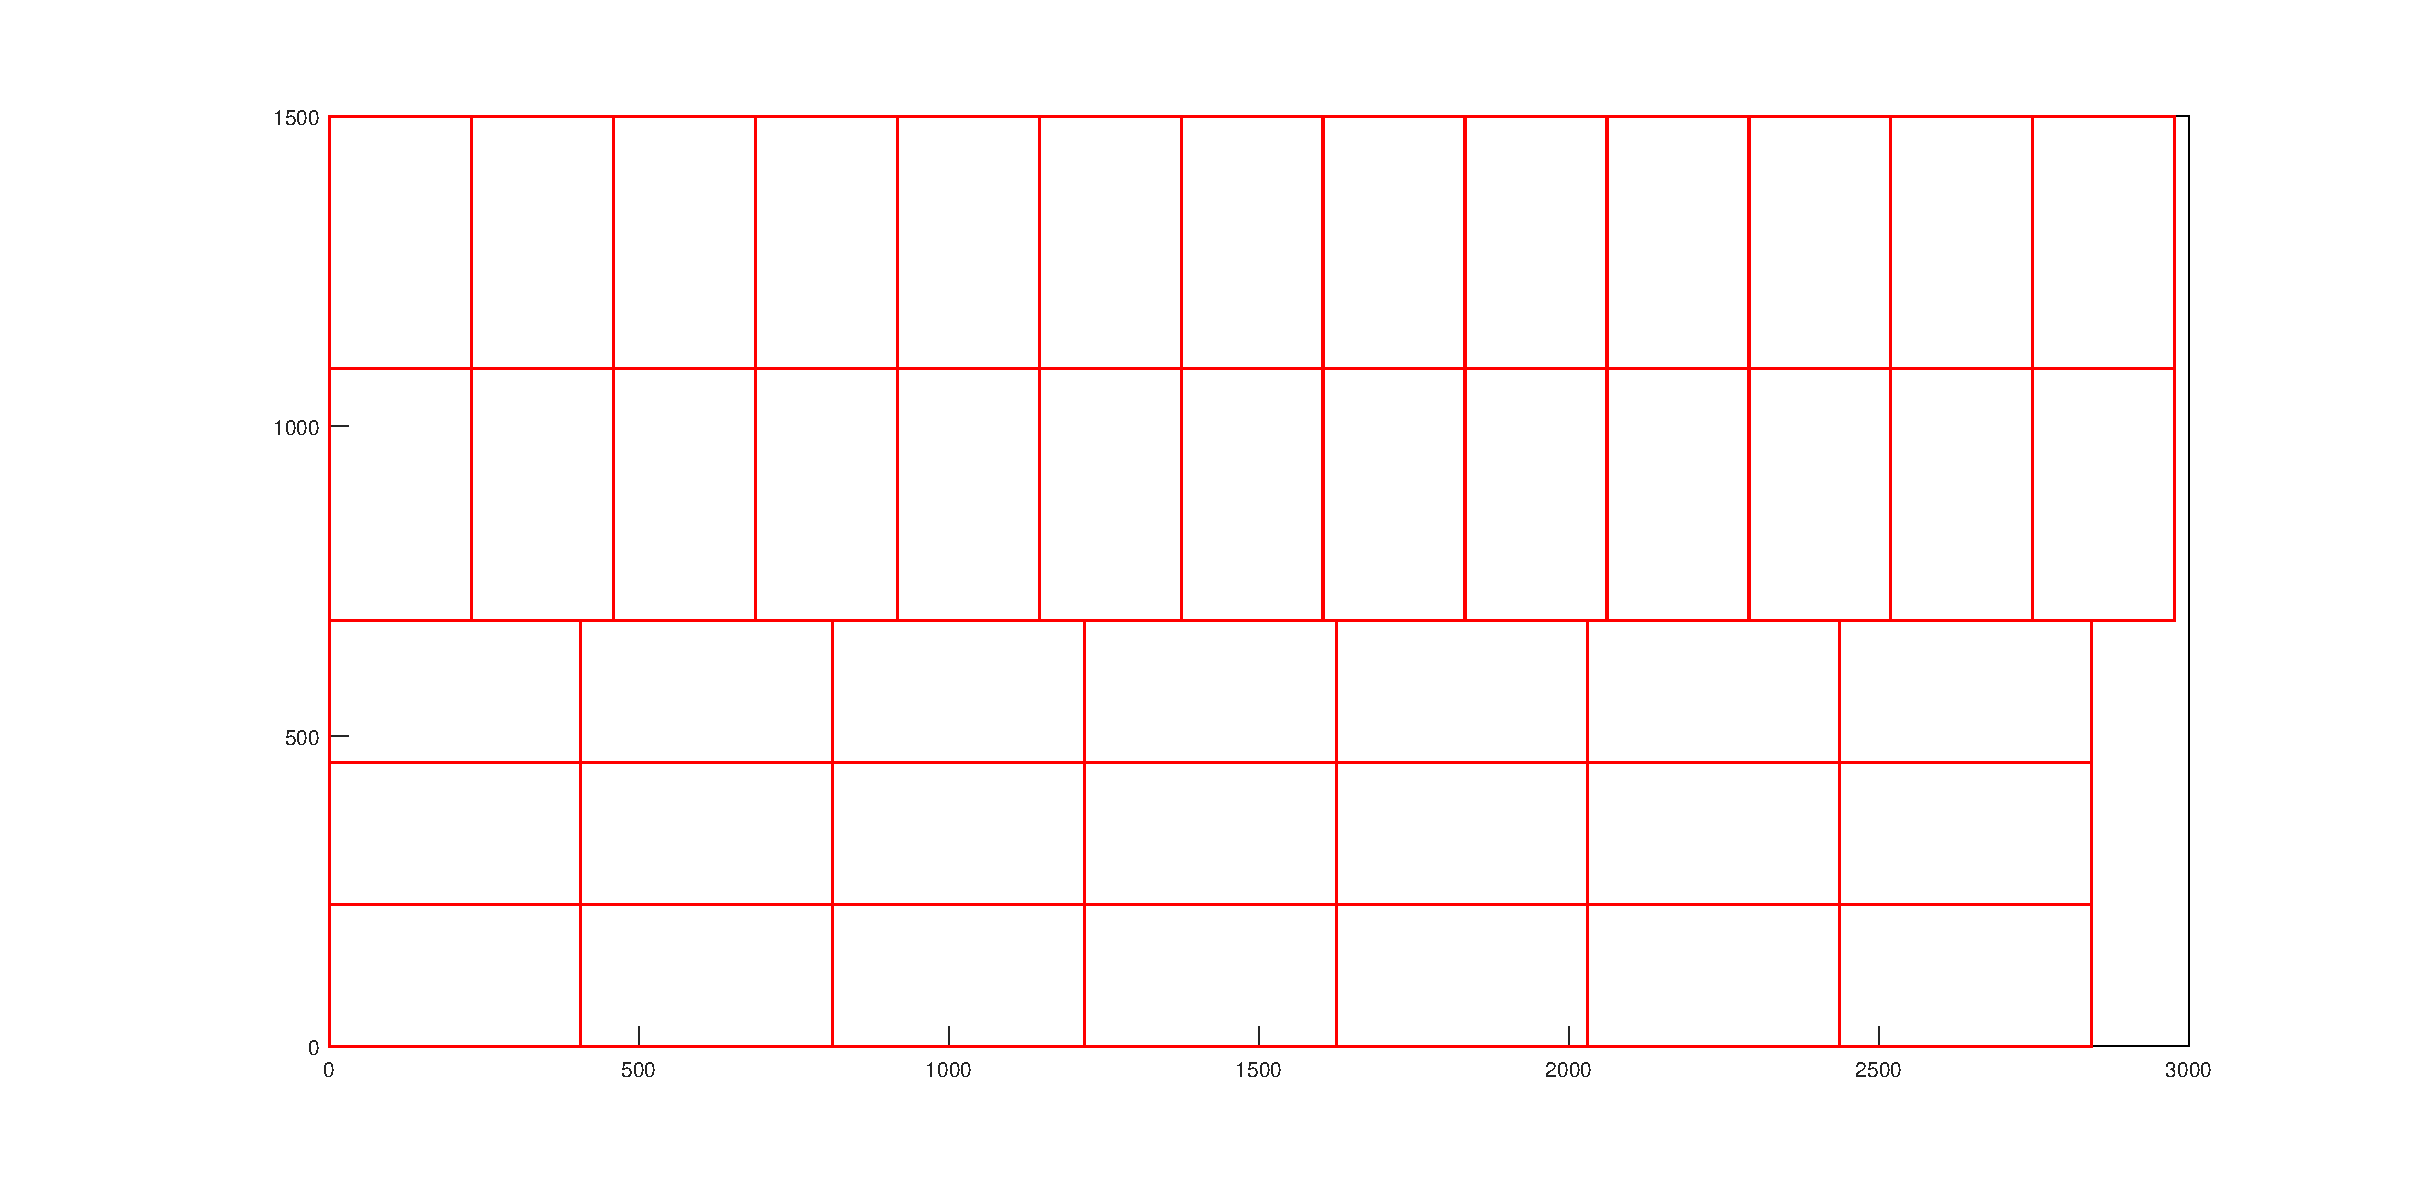
\includegraphics[width=\textwidth]{picture/P_1_3}
  \caption{问题三$k_5$切割方案图示 }\label{qiegex3}
\end{figure}
\paragraph{问题四的模型建立与求解}
同理设决策变量 $k_i$为按第i种方案切割的木板块数($i=1,2,\cdots,25$),则目标函数为使用木板原材料的最小值,由表\ref{tab:haoliyong},设:
\begin{equation}\label{shuju1}
  A=\left(
            \begin{array}{cccc}
              3 & 5 & 27 & 15 \\
              0 & 2 & 45 &0 \\
              \vdots & \vdots & \vdots &\vdots \\
              0 & 24 & 6 & 8 \\
              20 & 21 & 0 & 0 \\
            \end{array}
          \right)
\end{equation}
\begin{equation}\label{shuju2}
          K=\left(
              \begin{array}{c}
                k_1 \\
                k_2 \\
                \vdots \\
                k_{25} \\
              \end{array}
            \right)
\end{equation}
于是,
\begin{equation}\label{zuixiaozhi2}
  \begin{split}
&\min \,\, N=\sum_{i=1}^{25} k_i\\
&s.t.\quad  \left\{\begin{array}{c}
A^TK\geq \left(
           \begin{array}{c}
             774 \\
             2153 \\
             1623 \\
             1614 \\
           \end{array}
         \right)
\quad \\
k_i\geq0\mbox{且为整数}\quad \\
\end{array}\right.
\end{split}
\end{equation}\par
用Matlab对该整数线性规划问题求解,得到最优解为:$k_4=3,k_7=57,k_{19}=49,k_{24}=31$
 ,其余为0,最小使用木板数N为140。\par 于是问题四的结果见表\ref{tab:quastion4}
\begin{table}[htbp]
  \centering
  \caption{\textbf{问题四的结果}}
    \begin{tabular}{|c|c|c|c|c|c|c|}
    \hline
    木板S1 & P1 &P2&P3 &P4& 木板 &\multicolumn{1}{c|}{\multirow{2}[0]{*}{备注}} \\\bigstrut
    的数量&的数量&的数量&的数量&的数量&利用率&\\\hline
    3 & 40 & 5 & 6 & 3 & 98.650\% & 每块木板切割方案相同\\\hline
    57 & 12 & 9 & 25 & 0 &98.548\% & 每块木板切割方案相同\\\hline
    49 & 0 & 18 & 0 & 28 & 97.346\% & 每块木板切割方案相同 \\\hline
    31 & 0 & 24 & 6 & 8 & 96.577\% & 每块木板切割方案相同 \\\hline
    合计数量:  & \multicolumn{1}{c|}{\multirow{2}[0]{*}{774}} & \multicolumn{1}{c|}{\multirow{2}[0]{*}{2153}} & \multicolumn{1}{c|}{\multirow{2}[0]{*}{1623}} & \multicolumn{1}{c|}{\multirow{2}[0]{*}{1614}} & 木板总利用率: &\multicolumn{1}{c|}{\multirow{2}[0]{*}{木板总利用率=$\frac{\mbox{所有产品的总面积}}{\mbox{所有木板的总面积}}$}}\\
    140&           &      &      &      &   97.059\%   &                                 \\\hline
    \end{tabular}%
  \label{tab:quastion4}%
\end{table}%

 以蓝色矩形代表P1,绿色矩形代表P2,红色矩形代表P3,紫色矩形代表P4,得到P1、P2、P3、P4在S1上的排样图见图\ref{qiegexx1}
 至图\ref{qiegexx4}
 。
 \begin{figure}[htbp]
  \centering
  \includegraphics[width=\textwidth]{picture/P3_1}
  \caption{问题四$k_4$切割方案图示 }\label{qiegexx1}
\end{figure}
\begin{figure}[htbp]
  \centering
  \includegraphics[width=\textwidth]{picture/P3_2}
  \caption{问题四$k_7$切割方案图示 }\label{qiegexx2}
\end{figure}
\begin{figure}[htbp]
  \centering
  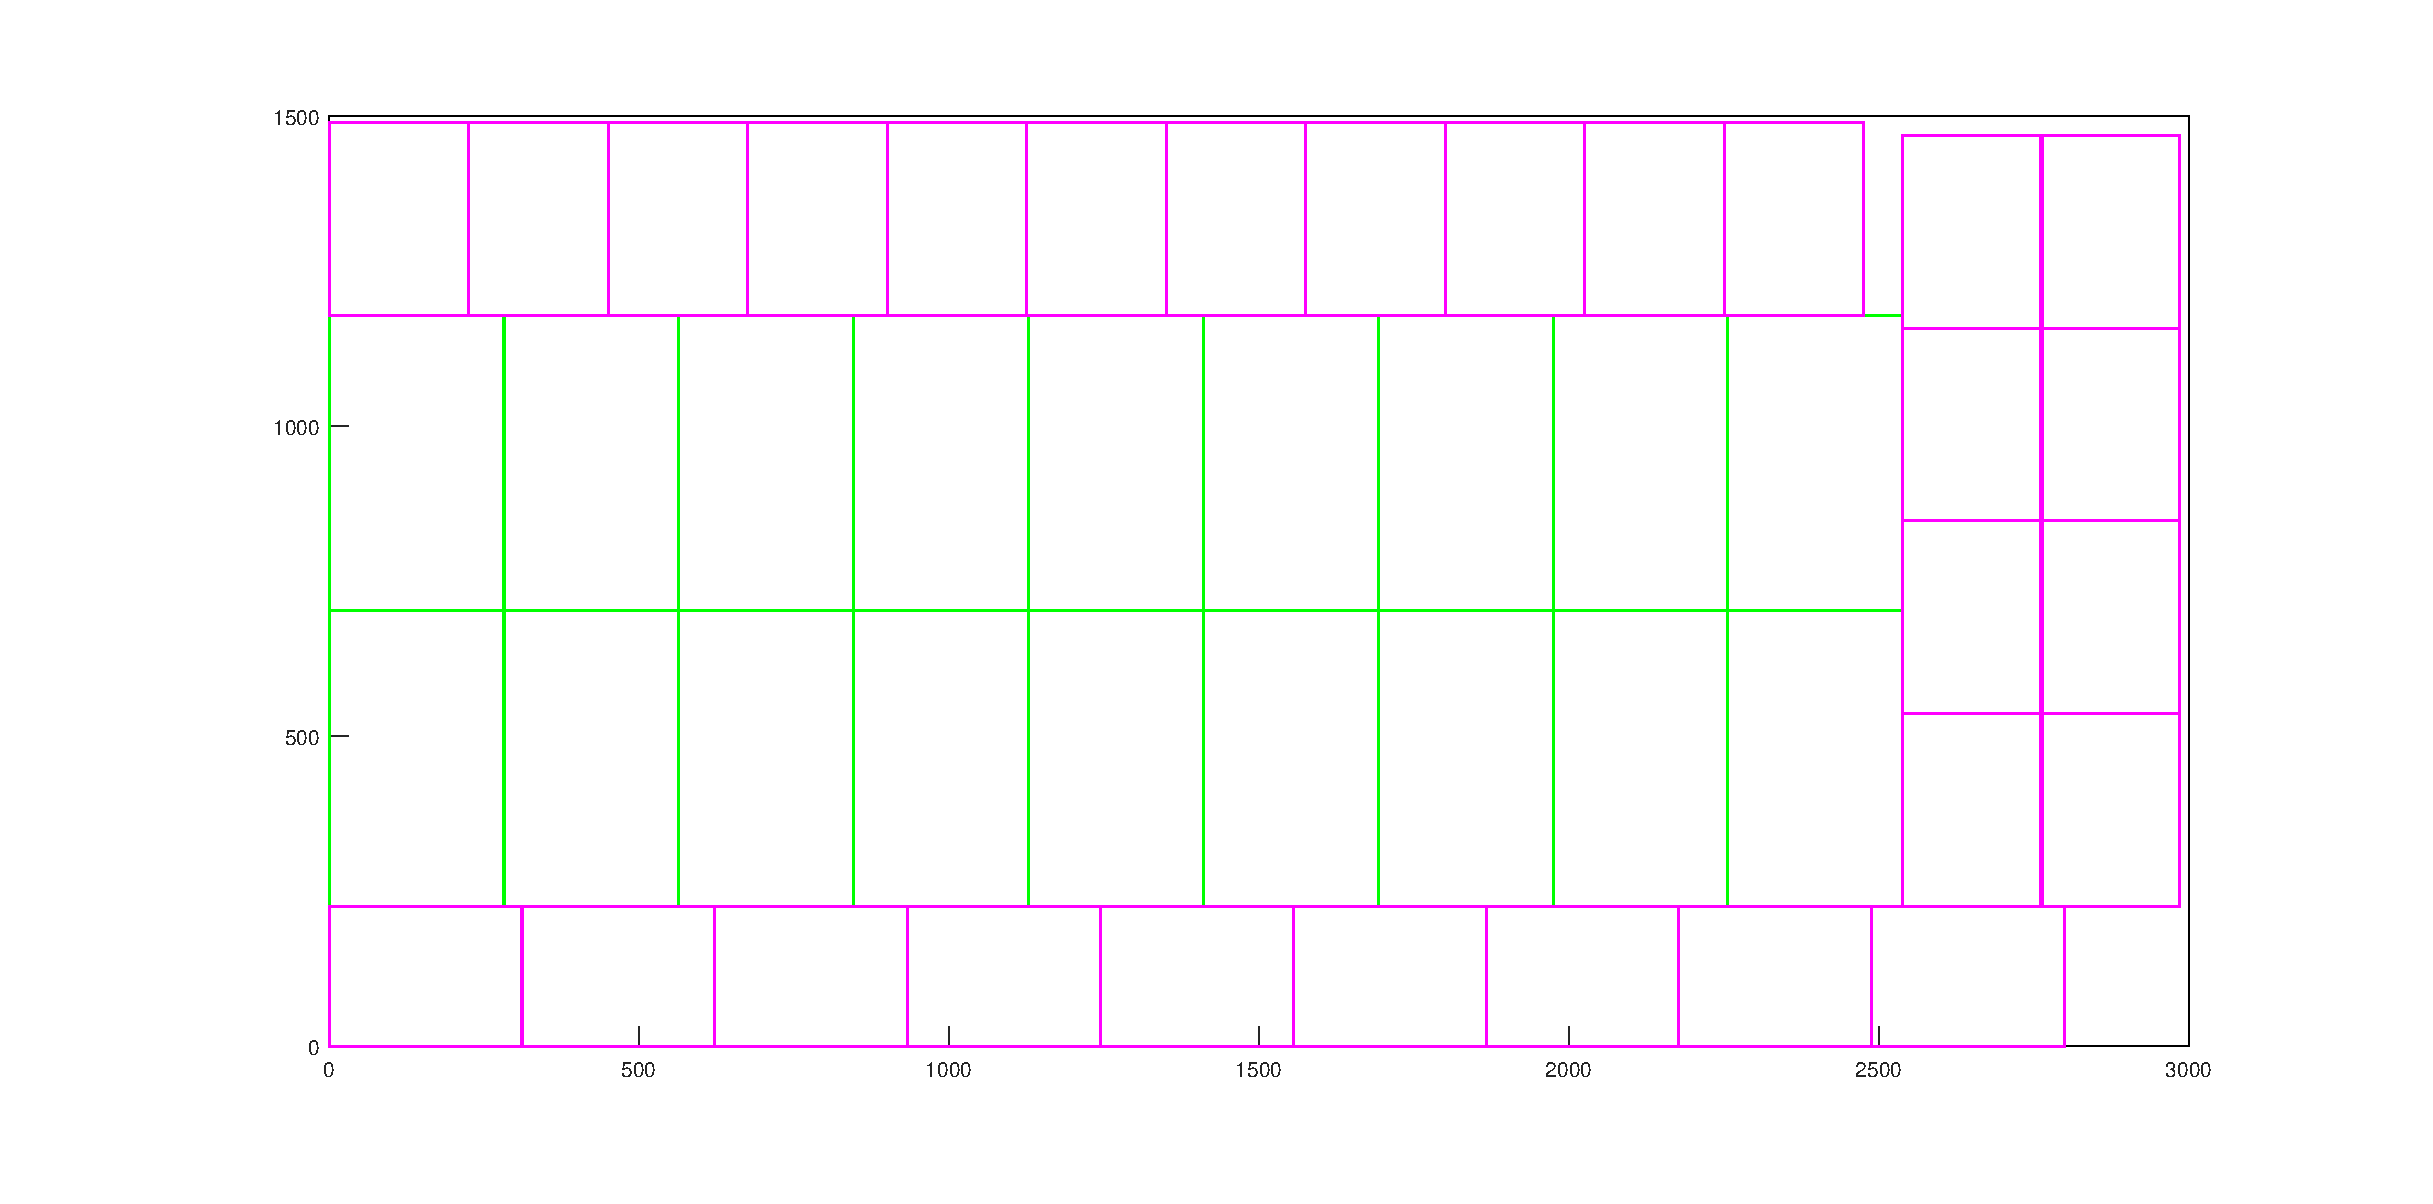
\includegraphics[width=\textwidth]{picture/P3_3}
  \caption{问题四$k_{19}$切割方案图示 }\label{qiegexx3}
\end{figure}
\begin{figure}[htbp]
  \centering
  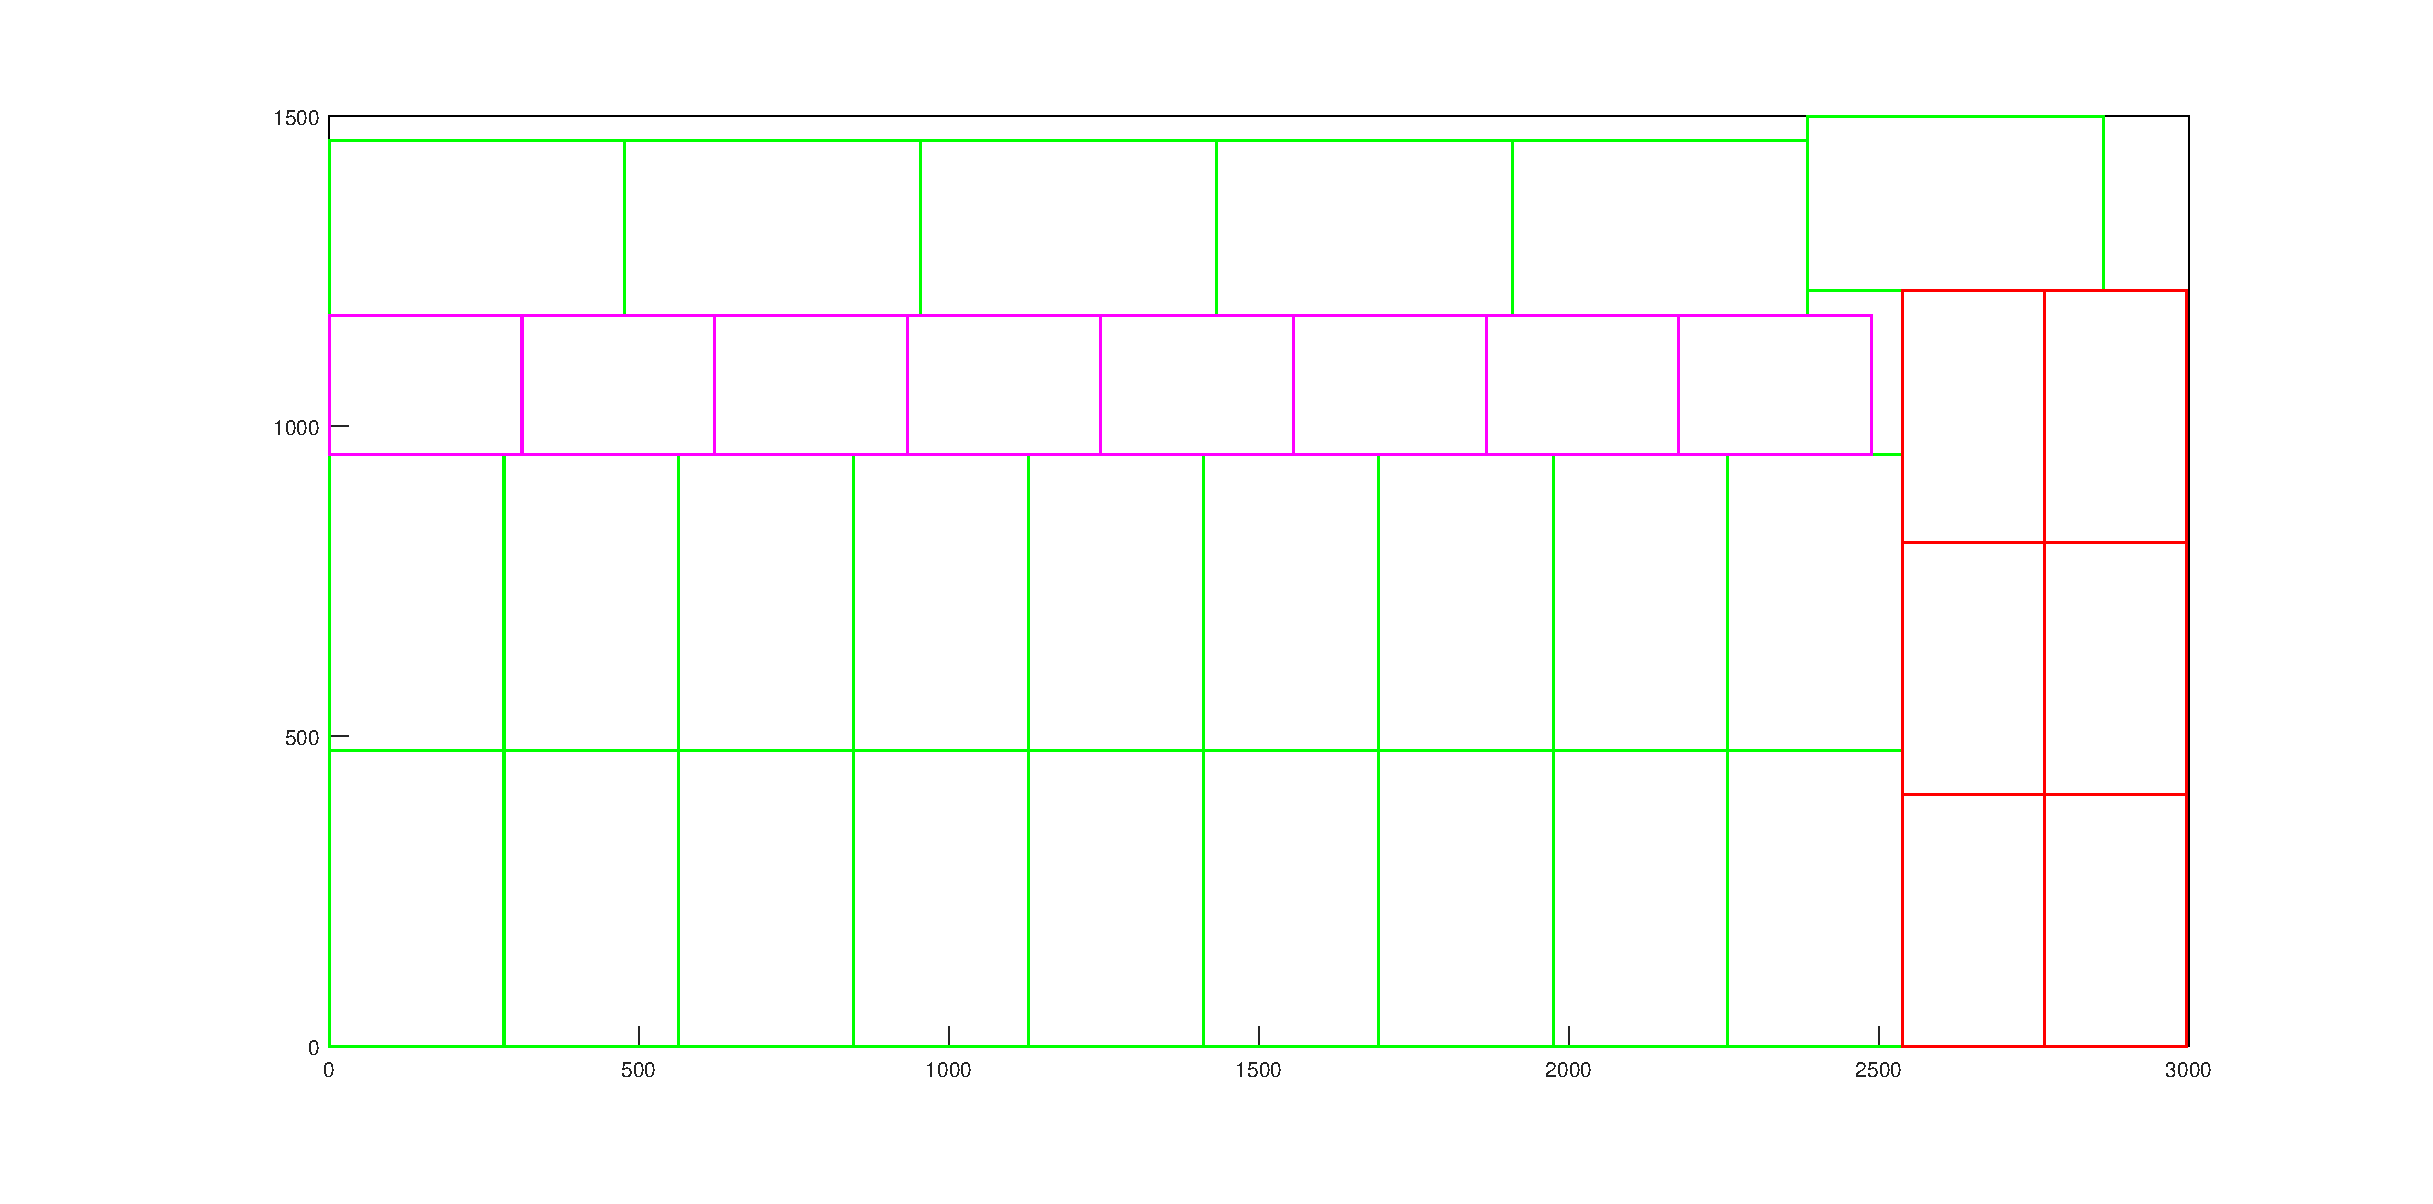
\includegraphics[width=\textwidth]{picture/P3_4}
  \caption{问题四$k_{24}$切割方案图示 }\label{qiegexx4}
\end{figure}
\subsection{问题五的问题分析与求解}
\subsubsection{问题分析}
第五问对100块S1木板进行切割,对P1、P2、P3、P4的数量不作要求,只要总利润最大。四种产品的面积不同,用100块S1切割出来的数量也不同,单件产品所获利润也不同。而 总利润$=$产品数量$\times$单件产品利润,要使总利润最大需使切割的数量及其单件利润都较大。根据问题四的分析得到25种在一块木板上切割P1,P2,P3,P4的高利用率方案,木板利用率越高则意味着在S1上切割得到的产品数量越多。我们仍然对这25种高利用率方案进行组合,利用整数线性规划求得总利润最高时的切割方案。
\subsubsection{模型的建立与求解}
设决策变量$k_i$为按第i种方案切割的木板块数($i=1,2,\cdots,25$),沿用式(\ref{shuju1})、式(\ref{shuju2}),并设:
\begin{equation}\label{shuju3}
  A^TK=\left(
         \begin{array}{c}
           n_{P1} \\
           n_{P2} \\
           n_{P3} \\
           n_{P4} \\
         \end{array}
       \right)
\end{equation}
记总利润为M,
\begin{equation}\label{zuixiaozhi3}
\begin{array}{c}
  \max  M=19.9\times n_{P1}+23.0\times n_{P2}+21.0\times\ n_{P3}+16.0\times\ n_{P4} \\
  s.t. \sum_{i=1}^{25}k_i\leq 100
\end{array}
\end{equation}
用Matlab对该整数线性规划问题求解,得到最优解为$k_8=100$,其余为0,N=100。
即100块S1全部切割成P1产品获得的总利润最大。\par
于是,问题五的结果见表\ref{tab:quastion5}
。
% Table generated by Excel2LaTeX from sheet 'Sheet10'
\begin{table}[htbp]
  \centering
  \caption{\textbf{问题五的结果}}
    \begin{tabular}{|c|c|c|c|c|c|c|c|}
    \hline
    木板S1 & P1 & P2 & P3 & P4 & \multirow{2}[0]{*}{利润} & 木板 & \multirow{2}[0]{*}{备注} \\
    的数量 & 的数量 & 的数量 & 的数量 & 的数量 &   & 利用率 &  \\\hline
    100 & 5900 & 0 & 0 & 0 & 117410 & 98.298\% & 每块木板切割方案相同 \\\hline
    木板S1 & \multirow{3}[0]{*}{5900} & \multirow{3}[0]{*}{0} & \multirow{3}[0]{*}{0} & \multirow{3}[0]{*}{0} & 总利润: & 木板 & 木板总利用率 \\
    \multirow{2}[0]{*}{合计数量100} &   &   &   &   & \multirow{2}[0]{*}{117410} & 总利用率: & \multirow{2}[0]{*}{=$\frac{\mbox{所有产品的总面积}}{\mbox{所有木板的总面积}}$} \\
      &   &   &   &   &   & 98.298\% &   \\\hline
    \end{tabular}%
  \label{tab:quastion5}%
\end{table}%


\section{模型检验与分析}
\subsection{假设的合理性分析}
\begin{enumerate}
\item 假设1排除了无关损耗对模型的影响;
\item 假设2简化由于切割工具带来的微小差异,使得模型更精确;
\item 假设3使矩形的任意不重合排样成为可能;
\item 假设4使模型的所有数据真实可靠;
\end{enumerate}
\subsection{可靠性分析(给出模型的使用范围)}
本文以剩余矩形匹配法为基础,针对不同的问题,引入不同的约束函数,以达到求解最高的木板利用率或最大利润
的最优算法模型。借助模拟退火的方法,实现全局最优解的寻求,模型的结果更加可靠。结合整数线性规划法,结果更真实。

此模型经过合理改进之后可以适用于各类制造业的排样及最优方案设计,最高利润的预估等各种问题,具有相当广泛的适用范围。

\subsection{模型的合理性分析}
本文建立的模型充分考虑到了各种原始条件的相互制约关系,通过假设,
考虑原始数据的真实性与合理性,即原始条件以及数据的合理性。

同时,模型利用剩余矩形匹配法,根据不同问题,有针对性的引入目标函数,及约束条件,达到最高利用率或最大利润的求解,
即模型设计中算法过程以及求解过程的合理,可信。

最终的结果进行确认,借助模拟退火算法得出结果,即结果的合理性。




\section{模型的评价与推广}
\subsection{模型的优缺点分析}
\subsubsection{模型的优点}
\begin{enumerate}
\item 通过合理且适当的假设,首先去除了一些特殊因素的干扰,提升了计算结果的可靠性;
\item 采用剩余矩形匹配法,结合整数线性规划,大大提高了算法的计算能力和结果可信度。
启发式的概率搜索方式不容易陷入局部最优,易于寻找到全局最优解。;
\item 针对不同的问题,引入不同的目标函数,对问题的适应性较好;
\end{enumerate}
\subsubsection{模型的缺点}
\begin{enumerate}
\item 基于高利用率的切割方案计算利润最优,有可能使得计算结果遗漏;
\item 虽然引入了约束函数,并且排除了一部分选项。但如果需要考虑的情况很多时,花费的时间可能较多。
\end{enumerate}

\subsection{模型的应用领域及推广}
本模型经过改进后,可用于各类制造业的下料问题,减少原料浪费,降低企业生产成本。其中,对于最大利润的计算模型,有助于企业合理安排生产计划,提高利润。
\newpage
\begin{thebibliography}{99}
\addcontentsline{toc}{section}{参考文献}
\bibitem{1}曾凤华,剩余矩形匹配算法在矩形件排样中的应用,机电工程技术,第35卷第3期:2006年,64-65。
\bibitem{2}全雪峰,沈继涛,基于模拟退火剩余矩形算法的矩形件排样,超星期刊,第37卷第3期:2016年,27-29。
\end{thebibliography}
\newpage
\appendix
\section{附录}
\subsection{原始数据}
木板尺寸见表\ref{xinxi1},产品尺寸及生产任务见表\ref{xinxi2}。
\begin{table}[htbp]
  \centering
  \caption{木板的尺寸}\label{xinxi1}%
% Table generated by Excel2LaTeX from sheet 'Sheet9'
% Table generated by Excel2LaTeX from sheet 'Sheet9'
\begin{tabular}{|c|c|c|}
\hline
木板 &长度(mm)&宽度(mm)\\
\hline
S1 & 3000 & 1500 \\
\hline
\end{tabular}%

\end{table}%


\begin{table}[htbp]
  \centering
  \caption{产品尺寸及生产任务}\label{xinxi2}%
    % Table generated by Excel2LaTeX from sheet 'Sheet9'
\begin{tabular}{|c|c|c|c|c|}
\hline
产品名称 & 长度(mm)& 宽度(mm) &生产任务(件) & 利润(元/件)\\
\hline
P1 & 373 & 201 & 774 & 19.9 \\
\hline
P2 & 477 & 282 & 2153 & 23 \\
\hline
P3 & 406 & 229 & 1623 & 21 \\
\hline
P4 & 311 & 225 & 1614 & 16 \\
\hline
\end{tabular}%

\end{table}%
\newpage
\subsection{Matlab模型源代码}
\subsubsection{问题一、二的代码}
\begin{lstlisting}
clear
board_size = [3000, 1500];
%Primitive arrangement of product dimensions
S0=zeros(60+48,2);
for i=1:60
    S0(i,1)=373;
    S0(i,2)=201;
end
% for j=48:48+60
%     S0(i,1)=406;
%     S0(i,2)=229;
% end

% constants

% Temperature drop using Lundy and Mess formula
d_0 = 1;           %According to the definition of f
K = 10;
t0 = K * d_0;    %initial temperature
tf = 10;
M = 50000;         %Upper limit of total iteration times
beta = (t0-tf) / (M*t0*tf);

%
L = 200;                 %Lower bound of iteration times at the same temperature
U = 500;                %The Upper Bound of iteration times at the Same Temperature
Accept_Ratio = 0.5;
%Ratio of the number of iterations accepted to the number of iterations at the same temperature


S = S0;                 % Initial solution
i_Iter = 2;               % times of iterations at the same temperature
nTotal_Iter = 0;      % Total times of iterations

k = 1;                    % times of iterations at different temperatures
ratio(k) = 1;           % Cost function: ratio of surplus to total consumption
tk(1) = t0;              % Temperature
fmin = 1;        % Minimum Cost Function
solution = S;              % optimum solution

while( nTotal_Iter<M && fmin > 0.02  )

    i_Iter = 0;
    iAccept_Iter = 0;
    fS = f( S, board_size, false );
    while ( i_Iter<U )

         Sstar = N( S );
         df = 0;
         fStar = f( Sstar, board_size, false);
         df = fStar - fS;

         if ( df <=0 || exp( -df / tk(k) ) > rand )
             S = Sstar;
             fS = fStar;
             iAccept_Iter = iAccept_Iter + 1;
         end

         % When the temperature drops to the limit
         if fS < fmin
             fmin = fS;
             solution = S;
         end

         i_Iter = i_Iter + 1;
         nTotal_Iter = nTotal_Iter + 1;

         if ( i_Iter > L && iAccept_Iter/i_Iter > Accept_Ratio )
             fprintf('iAcceptIter/iIter = %f\n', iAccept_Iter/i_Iter);
             break;              %Temperature drop
         end

    end

    ratio(k) = f(S, board_size, false);

    fprintf('iOuterLoop = %d, iIter = %d, tk = %f, ratio = %f, fbestratio=%f\n', k, i_Iter, tk(k), ratio(k), fmin);

    %tk(k+1) = tk(k) / ( 1+beta*tk(k) );
    %Temperature drop
    tk(k+1) = 0.9 * tk(k);

    k = k + 1;

end

fmin = f(solution, board_size, true);
fprintf('best ratio = %f, nTotalIter = %d\n', fmin, nTotal_Iter);
\end{lstlisting}
\subsubsection{问题三的代码}
\begin{lstlisting}
clear
clc
f=[1 1 1 1 1 1 1];
ic=[1 2 3 4 5 6 7 ];
A=-1*[44 35 32 0 59 45 16;12 19 21 47 0 11 34];
b=[-774;-1623];
lb=zeros(7,1);
[x,fval]=intlinprog(f,ic,A,b,[],[],lb,[])
\end{lstlisting}
\subsubsection{问题四的代码}
\begin{lstlisting}
clear
clc
d=25;
f=ones(d,1);
ic=ones(d,1);
for i=1:size(ic,1)
    ic(i)=i;
end
A=-1*[3 0 0 40 1 24 12 59 0 0 36 0 45 48 10 0 33 0 0 16 9 0 0 0 20;
5 2 0 5 6 4 9 0 8 0 6 10 7 6 10 14 11 4 18 6 19 0 8 24 21;
27 45 41 6 36 0 25 0 36 43 6 33 1 0 0 12 1 12 0 24 4 47 0 6 0;
15 0 9 3 3 30 0 0 0 6 5 0 0 0 33 20 5 39 28 2 11 0 47 8 0;];
b=-1*[774;2153;1623;1614];
lb=zeros(d,1);
[x,fval]=intlinprog(f,ic,A,b,[],[],lb,[])
\end{lstlisting}
\subsubsection{问题五的代码}
\begin{lstlisting}
clear
clc
d=25;
NUM=[3 5 27 15 ; 0 2 45 0 ; 0 0 41 9 ; 40 5 6 3 ; 1 6 36 3 ; 24 4 0 30 ;
    12 9 25 0 ; 59 0 0 0 ; 0 8 36 0 ; 0 0 43 6 ; 36 6 6 5 ; 0 10 33 0 ;
    45 7 1 0 ; 48 6 0 0 ; 10 10 0 33 ; 0 14 12 20 ; 33 11 1 5 ; 0 4 12 39 ;
    0 18 0 28 ; 16 6 24 2 ; 9 19 4 11 ; 0 0 47 0 ; 0 8 0 47 ; 0 24 6 8 ; 20 21 0 0 ; ];
Prise=[19.9	23	21	16];
Profit=zeros(1,d);
for i=1:size(Profit,2)
    for j=1:size(Prise,2)
   Profit(i)=Profit(i)+NUM(i,j)*Prise(j);
    end
end
 f=-100*Profit;
 ic=ones(d,1);
 for i=1:size(ic,1)
     ic(i)=i;
 end
 A=ones(1,25);
 b=[100];
 lb=zeros(d,1);
 [x,fval]=intlinprog(f,ic,A,b,[],[],lb,[])
\end{lstlisting}
\end{document}
